\chapter{SaRoMaN}
%\chapter{Software development}
\label{c:software}

\section{Introduction}

The software environment used for Baby MIND is the SaRoMaN (Simulation and Reconstruction of Muons and Neutrinos) software suite which is a comprehensive software for MIND/nuSTORM detectors and has been developed at the University of Glasgow over several iterations~\cite{27Bross,  53Laing, 54NUFACT2016Hallsjo}. The software has been expanded to be able to model and simulate a generic detector with limitations in the current implementation of the reconstruction. It includes a complete range of functionality for simulating single particle beams, through GEANT4~\cite{Geant4} or neutrino beams, through GENIE~\cite{Genie}, including geometry design, digitisation and reconstruction through RecPack~\cite{RecPack}. The software suite is also shipped with several analysis code examples written in ROOT~\cite{Root}. It has been created exploiting software engineering and object-oriented technology and implemented in the C++ and Python programming languages. The software is accessible on request from \url{https://lspace.ppe.gla.ac.uk}. 

\section{General structure}
The SaRoMaN software suites main design goal has been to promote modularity, single point of entry and simplicity for the user. With this in mind the SaRoMaN software is split into four main parts which can be replaced or altered independently of the others as long as the input/output flow is conserved. The parts are denoted, wrapper, simulation, digitisation and reconstruction with the flow seen in \FigRef{fig:codeFlow} and a more detailed view in \FigRef{fig:structure}. Each part will be discussed further below.

\begin{figure}[h!]
\centering
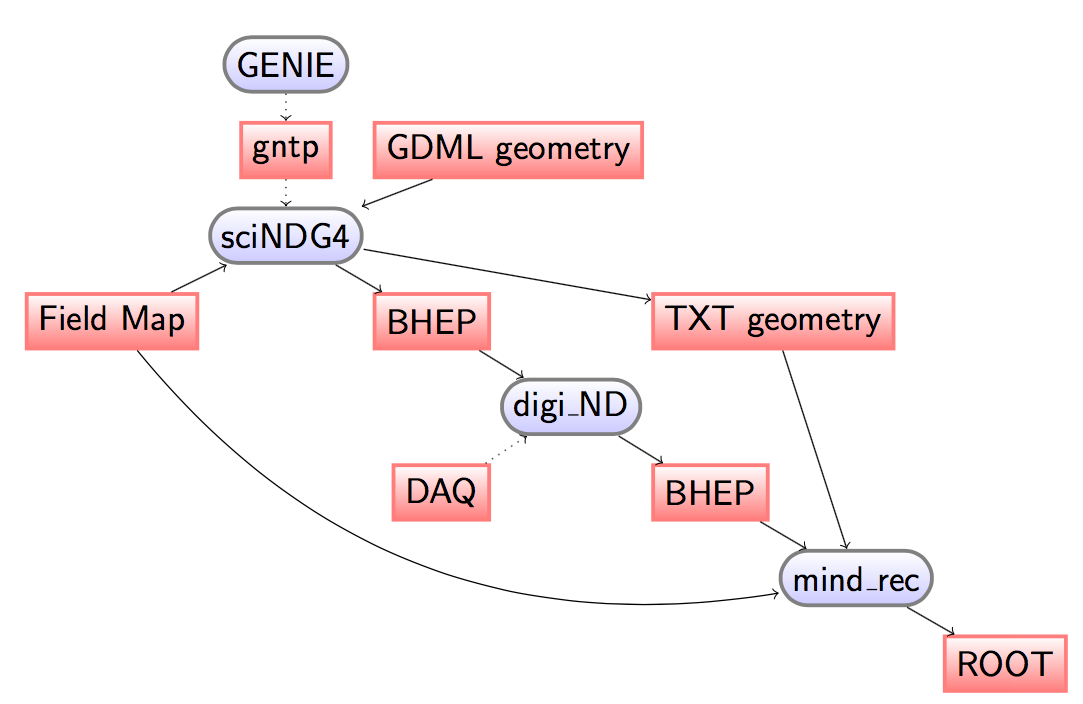
\includegraphics[width=\textwidth]{figures/codeFlow.png}
\caption{Code flow of the SaRoMaN software suite all controlled and handled through a wrapper.}
\label{fig:codeFlow}
\end{figure}

\begin{figure}[h!]
\centering
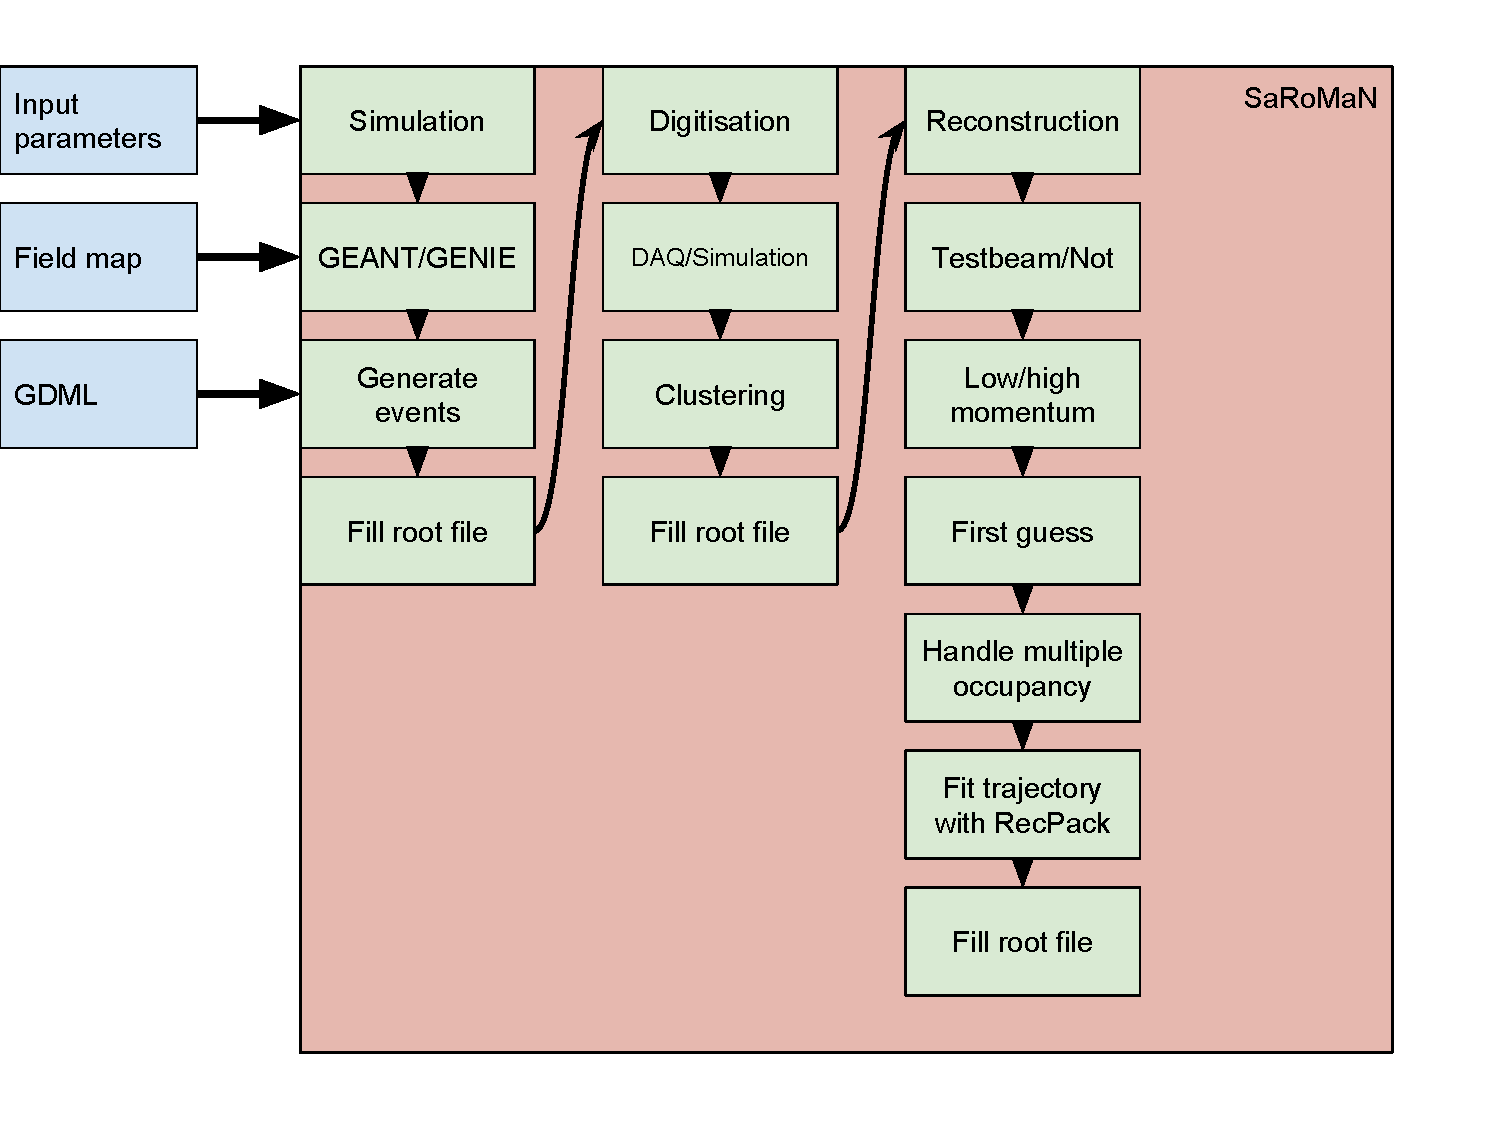
\includegraphics[width=\textwidth]{figures/Software_structure.pdf}
\caption{Code structure of the SaRoMaN software suite all controlled and handled through a wrapper.}
\label{fig:structure}
\end{figure}

%The second simulation etc etc.
%Add diagram of code, structure etc. Perhaps some code and or file structures in the appendix.
%Plot the overlaying idea and structure. Stress modularity, charge, momentum and particle type

\section{Wrapper}
To simplify the installation, compiling and usage of the other parts in the SaRoMaN suite, a wrapper has been developed in the Python programming language. This wrapper, aside from the above, handles all input variables, file names, writing of configuration files, standardisation of magnetic field map and geometry, and data flow between the other parts. 

To simplify for the user, all of the installation, compilation and running are handled through simple command line inputs with the option of more advanced commands being issued through the use of the Python wrapper class. After installation SaRoMaN can be run with some default parameters, a full run diagram can be seen in \FigRef{fig:block}.

\begin{figure}[h!]
\centering
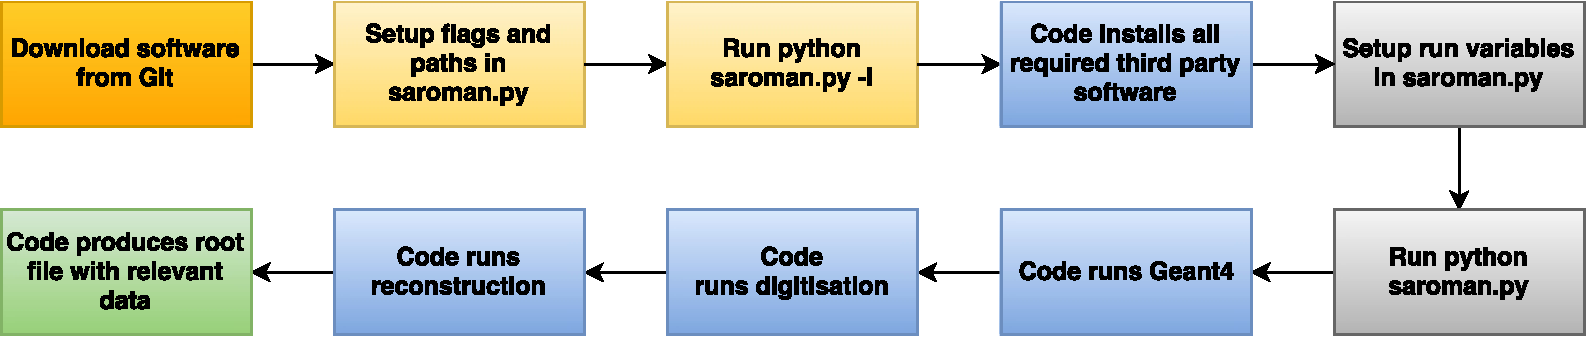
\includegraphics[width=\textwidth]{figures/block.pdf}
\caption{Example of how to run a default simulation.}
\label{fig:block}
\end{figure}

\section{Simulation}
Simulations are used to model how particles will interact with a detector model and what scintillator hits can be expected. The outputs from the simulation include the position of the hit on a bar, the location of a bar, the time of the hit and the amount of energy that was deposited.

The simulation comes with two different modes, neutrino or "single particle". For neutrinos GENIE is first run to generate neutrino events. These events are later populated and the detector constructed through GEANT. In a single particle mode a beam of a single particle type is assumed, GENIE is not called and the simulation and detector construction are handled through GEANT.

A unique feature is that the whole SaRoMaN suite uses a single geometry definition for the whole suite, written in Geometry Description Markup Language (GDML)~\cite{GDML} which is interpreted in GEANT and passed as a simplified .txt file to the reconstruction, which simplifies any changes of the geometry. 

\section{Digitisation}
Digitization is the emulation of the hardware required to build the detector. It needs to handle the response of the electronics and describes the expected output signals, based on input hits in the detector. This is currently done in a simplified way by smearing data with different Poisson distributions as well as handling events which are distinguished by a large time difference. For the Baby MIND detector the algorithms take the horizontal and vertical bar hits and clusters together hits to construct x, y and z positions along with the energy deposition and time to produce physical hit points. The full program flow can be seen in \FigRef{fig:digi}.

As a way to simplify the integration and implementation, the data acquisition (DAQ) used for the different test beams have been implemented in the digitisation as well. In this mode, real data is given as input and only the clustering takes place. Due to the usage of a single geometry, a token simulation has to be run in this mode as well to properly construct the geometry.

To ensure that all further analysis is performed properly, there is no way to distinguish data coming out of the digitisation as being simulated or read in through the DAQ.

One of the most difficult design features of Baby MIND is combining hits from both vertical and horizontal bars. It is possible to get hits which can not be combined without ambiguity. In figure~\FigRef{fig:BarAmbi} it is impossible to distinguished the green hits from each other and the same with the red hits. The current method is for the digitisation to create both hits at all times and these hits being handled by the reconstruction.

\begin{figure}[h!]
\centering
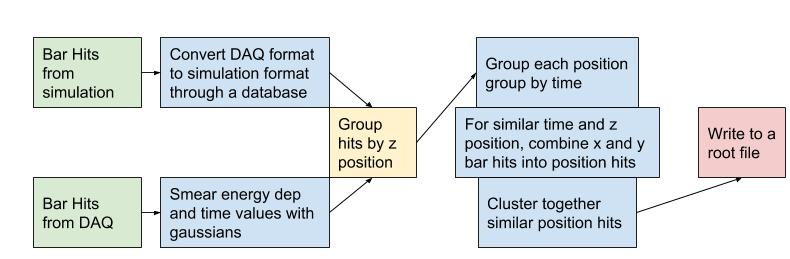
\includegraphics[width=\textwidth]{figures/Digitisation.jpg}
\caption{Program flow for the digitisation.}
\label{fig:digi}
\end{figure}

\begin{figure}[h!]
\centering
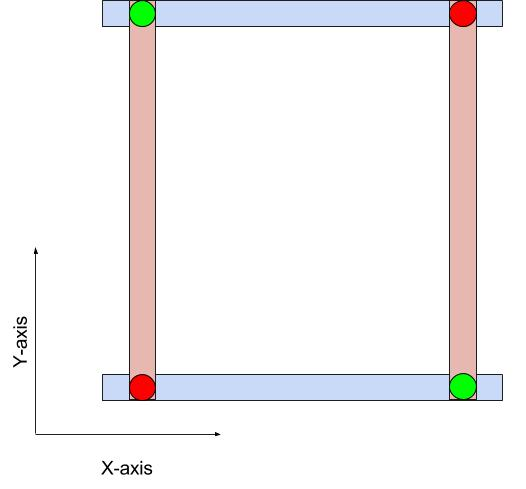
\includegraphics[width=0.5\textwidth]{figures/BarsAmbi.jpg}
\caption{}
\label{fig:BarAmbi}
\end{figure}

\subsection{Simulated data}

The digitisation is provided with a .root file containing the following variables, add list? 

Given that the data is assumed to be analysed offline, the first task is to separate any hits into event time windows, where hits can be seen as coming from the same particle. The main difficulty is to allow for the particle to fully traverse the detector and allow delay in electronics response in the time window. This provides a number of hits in several time bins, denoted as events without having use the position information. Add plot, logical flow chart.

After the timing clustering so called 3-d space points are created by combining the vertical and horizontal bar hits for a specific module. These three points are combined to provide an x,y and z coordinate. In this bar coincidence as well as overlap are taken into account as mentioned previously by creating all of the possible points. For this position clustering energy is combined between the individual hits to create a or several clusters with a discrete position, based on bar overlap, deposited energy and time.

The final step in the digitisation is to smear the value of deposited energy and hit time based on measured values of propagation time through the scintillator bars given the simulated hit position and not only the bar position.

\subsection{DAQ}
\textbf{Here or test beam?}

The current DAQ framework for the Baby MIND detector is based on being used offline, processed both after and away from the acquisition.

For simplicity the DAQ converts the acquired data and converts it into the same format as expected from a simulation so that the digitisation can be used in the same way. The main difference is that the smearing used for simulated data is turned off. In this section the DAQ will be discussed. 

Data comes in with files specific for each FEB. This data, has channel number, hit time and hit amplitude. The first step is to convert the data into space-positions, either vertical or horizontal bar position information and z-position, using a database based on FEB, channel number and knowledge of the physical layout of the detector. The second step is ensuring that each hit position, time and amplitude. Step three is to cluster all of the hits in specific time slots, which are equivalent to the event time windows. When this is done several low level filters are performed, to ensure that an event has enough hits to produce atleast four 3-d space positions in a time slot. After these steps the data is equivalent to the data produced by a simulation.

\section{Reconstruction}
The reconstruction takes the digitized hit data and assembles tracks and vertices. The main physics parameters are the momentum as well as the charge of the particle. The main problems occur when there are overlapping hits with multiple occupancy per bar. In this situation, it is difficult to distinguish between valid hits and to extract the momentum of the track and its charge.
The first problem is handled by removing and adding hits and using a $\chi^2$ analysis through a Kalman fitter package, RecPack~\cite{RecPack}, to find the best trajectory that fits all hits.The second problem is solved through various algorithms to estimate the charge and momentum using different fits.

For simplicity the reconstruction currently contains a mode denoted as "test beam" where it does nothing more than writes out the input data into a final .root file.

\subsection{Structure}
The reconstruction software has been structured to ensure that the software is as modular as possible. It is currently based on the Kalman fitter package known as RecPack~\cite{RecPack} to provide both a framework and back bone for handling track objects. It is used for historical reasons, however SaRoMaN would benefit from using a Kalman fitter implementation which is still maintained, development, with few and understood bugs and has documentation.

A Kalman fitter is given an underlying model of the system, in our case knowing that particles travel as helices, and a model of the detector as well as other known inputs to the system to form an estimate of the different states in a way that is better than using only a single measurement. This is particularly well suited in particle physics where random noise is given through multiple scattering. It can also take into account the various energy losses and varying magnetic fields. Through this is can use measurements in different parts of the detector to estimate both how the particle has and will continue its propagation. Compared to other models, a Kalman fitter has no underlying assumption about the errors being Gaussian.

In high energy physics one frequently faces the problem of modeling the evolution of a dynamic system from a set of experimental measurements. Most of reconstruction programs use similar methods. However, in general they are reimplemented for each specific experimental setup. Some examples are fitting algorithms (i.e. Kalman Filter), equations for propagation, random noise estimation (i.e. multiple scattering), model corrections (i.e. energy loss, inhomogeneous magnetic field, etc.), model conversion, etc. Similarly, the data structure (measurements, tracks, vertices, etc.), which can be generalised as well, is not reused in most of the cases. The motivation for using RecPack comes from it combining all of this into a simple software package.

SaRoMaN has been split into first initializing the fitter, then using an initial pattern classification to choose reconstruction mode. Currently particles and showers are identified, but only muon-like particles are reconstructed. In this identification a track is produced along with any off track hits. Finally the fitter performs a final charge and momentum estimate on the track and tries to fit more tracks to the off track hits. If this is a neutrino sample, proton/neutron tracks are only built if it finds an initial muon track.

The test beam mode ignores the event classification and uses the fitter to pass information from input through to the final root file.

The reconstruction has split into several minor tasks.
\begin{itemize}
\item Handling data. Pushing the input data into a final root file.
\item Track building / pattern recognition, given an event, (a time window) can we build a track from this?
\item Fitting, with a candidate track, is it possible to add more hits to the track and make it longer? Find secondary tracks? Also, is it possible to estimate the momentum and charge of the track?
\end{itemize}

%How does the code work? When does the split happen? FitTrack in example Event by event. Goes on into fitter. split test beam or normal mode. Test beam only passes on the data with some minor calculations, straight line fit etc. Build planes. Fill planes with hits. After this, into classifier. In classifier, try to build trajectories. Find single "paths/tracks" if not, handle occupancy. Make a plot of this! Have all of the different modes here. Handle low and normal mode. Use or don't use recpack. Chi square analysis, add hits etc etc.  After classifier do a final fitter and write all of the data into a root file. For neutrinos handle short secondary tracks, atleast check for them. In the current implementation all parts use some part of RecPack. Stress modularity. Plot with flow through reconstruction.

\subsection{Pattern recognition}
The pattern recognition starts by looking at the number of hits for a given event. There are currently two main limitations to if a track can be fitted.
\begin{itemize}
\item At least 4 hit modules are required to do any form of charge estimation or track building.
\item At least 10 hit modules are required to perform a Kalman fitting.
\end{itemize}
Outside of these limitations, currently only muon track fitting has been implemented. The general assumption is that each even will contain at least one muon track followed by other secondary tracks. If this is not the case the event is discarded. The event filtering is done very simply by assuming anything that is not a shower is a muon. Single hits here refers to separable space points meaning that for each z-position there is only one unique hit. The aim of the pattern recognition is to find as many tracks with single hits as possible. In the pattern recognition track are built up from so called track stubs of at least 4 single hits. As soon as a track stub is created other hits can be added onto the track stub to create a final track using $\chi^2$ as a metric. This $\chi^2$ analysis is run through the fitter and requires an initial charge and momentum guess. This means that the best suitable hits are added to the track stub and the other hits saved for use in finding secondary tracks. 

The program flow can be seen as taking in an event worth of hits and returning a number of tracks along with hits which could not be fitted into any track. Each returned track contains only single hits as well as a momentum and charge estimate. The latter two are then improved by the fitter.

%Given an event, a time selection which can be seen as part of a accelerator spill cycle. Is it possible from the ensemble of hits to find a track or several tracks. Currently makes the assumption that tracks will be separable in space for at least 4 points or that there are 4 planes with single track points as to have an initial track to later add more points into.

\subsection{Fitting}
The fitters main job is to build tracks and to estimate the momentum and charge of that track. There are two modes, one main mode for hits with more than 9 hits are passed into the Kalman fitter RecPack. When it is not possible to perform a helical fit and for any track with more than 3 hits, a self implemented lever-arm approach is used. In both cases RecPack is used to build the tracks, however the momentum and charge reconstruction has to be split depending on the possibility of a helical fit or not. The full helix equation seen below, has a total of 9 parameters and takes 10 measurements to be fully fitted.  
\begin{align}
x(t) &= acos(bt+c)+d\\
y(t) &= esin(ft+g) + h\\
z(t) &= kt
\end{align}

The helix can be related to physical quantities as.
%This can also be written in a more helpful way as.
%http://www-jlc.kek.jp/subg/offl/lib/docs/helix_manip/main.html

\begin{align}
x(\phi) &= x_0 + d_p \cos \phi_0 + \frac{\alpha}{\kappa}(\cos \phi_0 - cos(\phi_0 + \phi))\\ 
y(\phi) &= y_0 + d_p \sin \phi_0 + \frac{\alpha}{\kappa}(\sin \phi_0 - cos(\phi_0 + \phi))\\
z(\phi) &= z_0 + d_z - \frac{\alpha}{\kappa} tan \lambda \phi
\end{align}
where $\vec{X} = (x_0, y_0, z_0)$ is the arbitrary helix pivot point, $d_p$ is the distance from the helix to the pivot point in the xy plane, $\phi_0$ is the azimuthal angle from the pivot point with respect tot the helix center, $\kappa$ is the signed reciprocal transverse momentum, $d_z$ is the distance of the helix from the pivot point in the z direction, and $\tan\lambda$ is the dip angle. The deflection angle $\phi$ is measured from the pivot point and specifies the position of the charged particle on the helical track. The variable $\kappa$ can be used to relate to the transverse particle momentum, $P_T$ and relate to the magnetic field as 
\begin{align}
 \kappa &=  Q/P_T \\  
 \rho &=  \alpha/\kappa
 \end{align}
where Q is the particle charge, $\rho$ being the signed radius of the helix, and $\alpha \equiv 1/c B$ being a magnetic-field-dependent constant with c as a constant and B the magnetic field strength. The full particle momentum can be obtained as 
\begin{equation}
\vec{P} = - \frac{Q}{\alpha} \frac{d\vec{X}}{d\phi} = \frac{1}{|\kappa |} 
 \begin{pmatrix}
 -\sin(\phi_0 + \phi)\\
 cos(\phi_0 + \phi)\\
 tan\lambda
 \end{pmatrix}
\end{equation}

In practice, this fit also takes both energy loss in the detector and multiple scattering into account when calculating the $\chi^2$ values when fitting the parameters. 

This motivates the requirement for two different modes. If a helical fit is possible RecPack performs the fitting and returns a final fitted helix, within provided measurement errors, with a momentum and charge estimate.

If a helical fit is not possible, denoted the low momentum case, several different algorithms are used.

The fitting is performed in a usual Kalman way by using this underlying equation and assuming each measurement point has some error.
Each measurement point $\vec{X}$ is related to the next through extrapolating the helical equation and assuming an error: $\vec{X_{k+1}} = \vec{F_{k+1,k}}\vec{X_k} + \vec{w_k}$. 
It is in this error term where multiple scattering and energy loss is taken into account.
The output is then given as: $\vec{Y_{k}} = \vec{H_{k}}\vec{X_k} + \vec{v_k}$
The helical equation goes into forming the matrix F and H.

Add note somewhere in how a helix is an approximation for our detector, we will have field, no field, straight line etc etc through the full detector.

\subsection{Low momentum algorithms}
The force applied to a particle travelling through a magnetic field is given by the Lorentz force:
\begin{equation}
\vec{F}=q\frac{\vec{v}\times\vec{B}}{c}
\end{equation}
where c is the speed of light in vacuum, v is the velocity, q the charge and B the magnetic field vector.

Using Newtons second law one produces the following differential vector equation.
\begin{equation}
\vec{F}=m\vec{a}=m\dot{\vec{v}}=q\frac{\vec{v}\times\vec{B}}{c}
\end{equation}
The solution to this equation is given by:
\begin{equation}
\vec{P}=m\vec{a}=m\vec{v}=q\frac{\vec{l}\times\vec{B}}{c}
\end{equation} 
where P is the momentum of the particle and $\vec{l}=\vec{X}-\vec{X_0}$ is a vector containing the lengths traversed through the magnetic field.

Using the definition of the cross-product, writing this as a scalar equation, using the small angle approximation and writing using S.I. units produces the normally recognisable equation
\begin{equation}
P = 0.3 QB_\bot \frac{|\vec{l}|}{\theta}=0.3 QB_\bot R
\end{equation}
where P is the momentum in MeV/c, the charge Q in in units of e, the magnetic field strength B is in T and the radius of curvature R is in cm. This is only one way of deriving the relation, but it is one of the main equations used for momentum reconstruction in SaRoMaN. The charge is then reconstructed using $P/|P|$. 

\begin{figure}[h!]
\centering
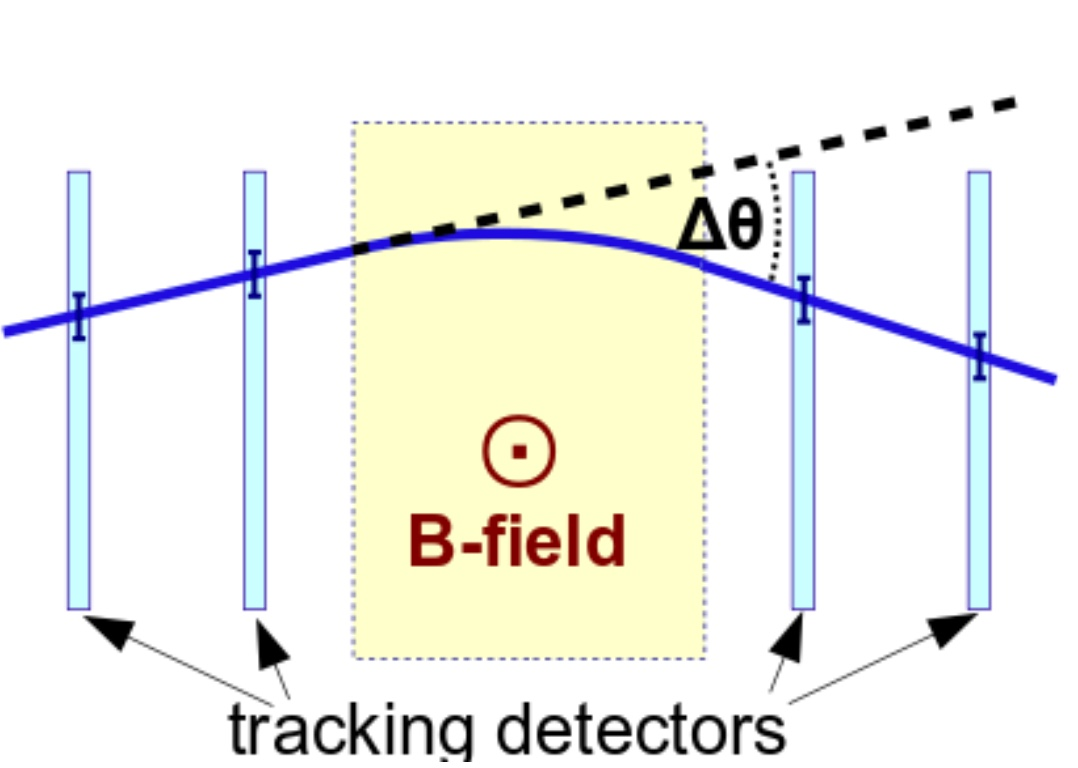
\includegraphics[width=0.5\textwidth]{figures/lowP/scattering.jpeg}
\caption{Figure of one bending in first plane in mind.}
\label{fig:Scattering}
\end{figure}

A previous study performed in the collaboration showed that the best best way of evaluating the charge comes from comparing both the first and second bending in the detector using two different distributions to handle the scattering.

\begin{figure}[h!]
\centering
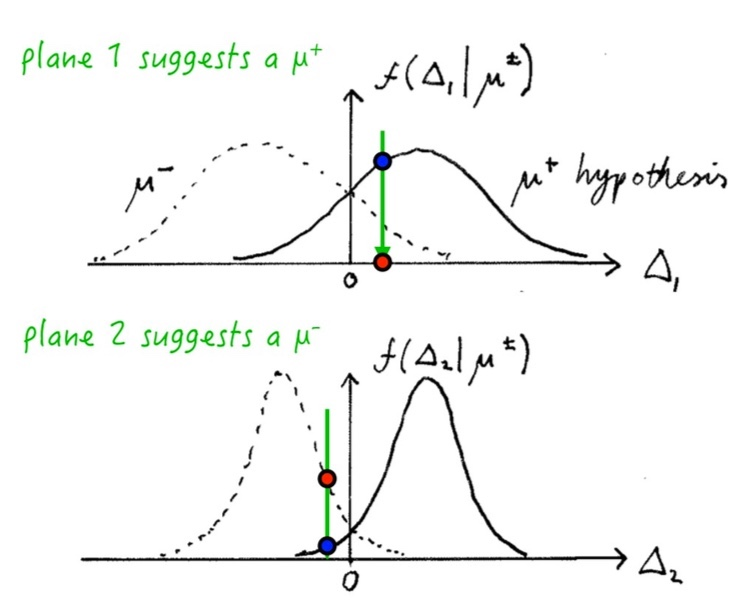
\includegraphics[width=0.5\textwidth]{figures/lowP/null.jpg}
\caption{}
\label{fig:NullHyp}
\end{figure}

Using the distribution of multiple scattering angles and the notation in \FigRef{fig:NullHyp}, the choice is taken as. 

Reconstruct $\mu^-$ if 
\begin{equation}
\frac{f_{\mu^-}(\Delta_1)}{f_{\mu^+}(\Delta_1)} > \frac{f_{\mu^+}(\Delta_2)}{f_{\mu^-}(\Delta_2)}
\end{equation}
and as $mu^+$ if
Reconstruct $\mu^-$ if 
\begin{equation}
\frac{f_{\mu^+}(\Delta_1)}{f_{\mu^-}(\Delta_1)} > \frac{f_{\mu^-}(\Delta_2)}{f_{\mu^+}(\Delta_2)}
\end{equation}

The bending angles are calculated from both measurement planes, (or only one if not possible) and tested against a null-hypothesis of having deflection from only multiple scattering 

%link from http://pdg.lbl.gov/2000/passagerpp.pdf
%Also, look at mind_rec/detector.c

multiple scattering  through small angles, the angle is given by, taken from pdg link
\begin{equation}
\theta_0 = \frac{13.6 MeV}{\beta cp} z \sqrt{x/X_0}[1+0.038\ln(x/X_0)]
\end{equation}
where p is the momentum, $\beta c$ the velocity, z the charge number of the incident particle and $x/X_0$ is the thickness of the scattering medium in radiation lengths.

The probability is calculated as 1/2pi exp -(scattering angle +- total bending angle) etc. check code.





Use the angles to and probability to calculate the charge. Momentum currently from range. Seems better.

Probability of angle from multiple scattering, or from magnetic field. 

Momentum comes from the range calculation, see detector layout. Major gaps in monument,  Potentially could and perhaps should use range momentum as long as tracks stop in detector. Problem with steps, helix better.

We have steps in the tracking detectors.

This seems to be the best approach. If this for some reason fails it goes on to a final attempt.

Quadratic fit, given few hits, try to fit to return charge. Use this only for charge. Momentum from range momentum.

\subsection{Performance}

\textbf{Add event display! also for testbeam in next chapter}

During development of SaRoMaN two main metrics were used to evaluate performance, charge reconstruction efficiency and track reconstructed efficiency. These metrics provide information about how many simulated tracks can be reconstructed and how many of those reconstructed tracks have the correct charge. This is done for muons of both charges and different momentum values.

Performance will be shown for the initial and proposed layout, for which the software algorithms were designed, the layout required for the text beam due to construction constraints and a final study based on the layout used for the WAGASCI detector layout. The main difference between the initial and test beam layout is removing the initial measurement point D0, restructuring  the layout and adding gaps between each of the blocks. This was done from a constructional not a physics motivation.

The charge identification is however improved when utilizing a measurement point from a neutrino target such as the WAGASCI, however this will reduce the lower limit of reconstruction since the muons must traverse the material of the WAGASCI. 

\textbf{Perhaps momentum rec plots as well? Look at old material/collaboration meeting 2 with pull and residuals.}
\textbf{One plot comparing all of these? Can we compare them? Lower momentum due to TASD?}

\begin{figure}[h!]
\centering
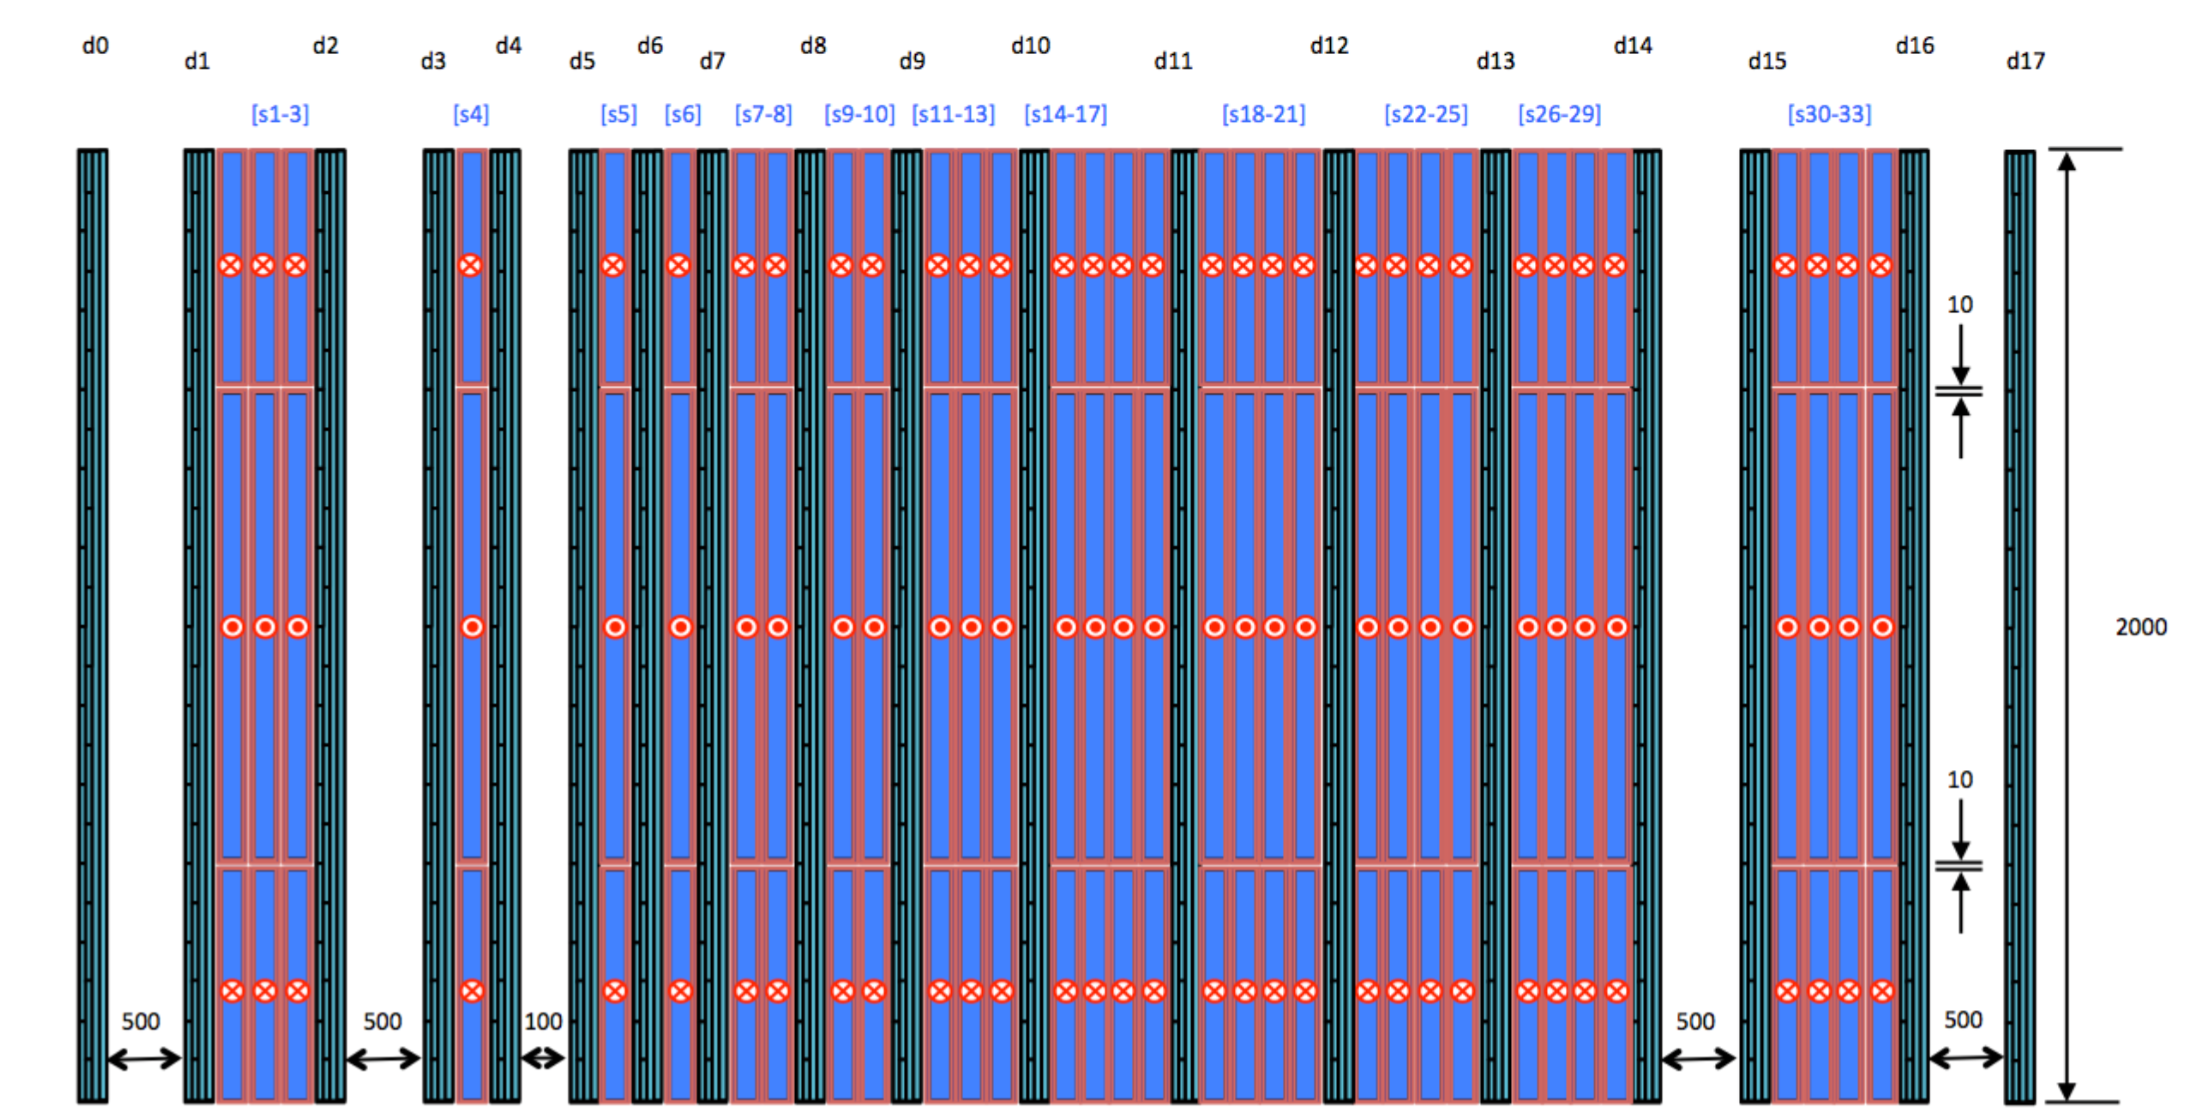
\includegraphics[width=0.48\textwidth]{figures/oldStudies/oldMIND.png}
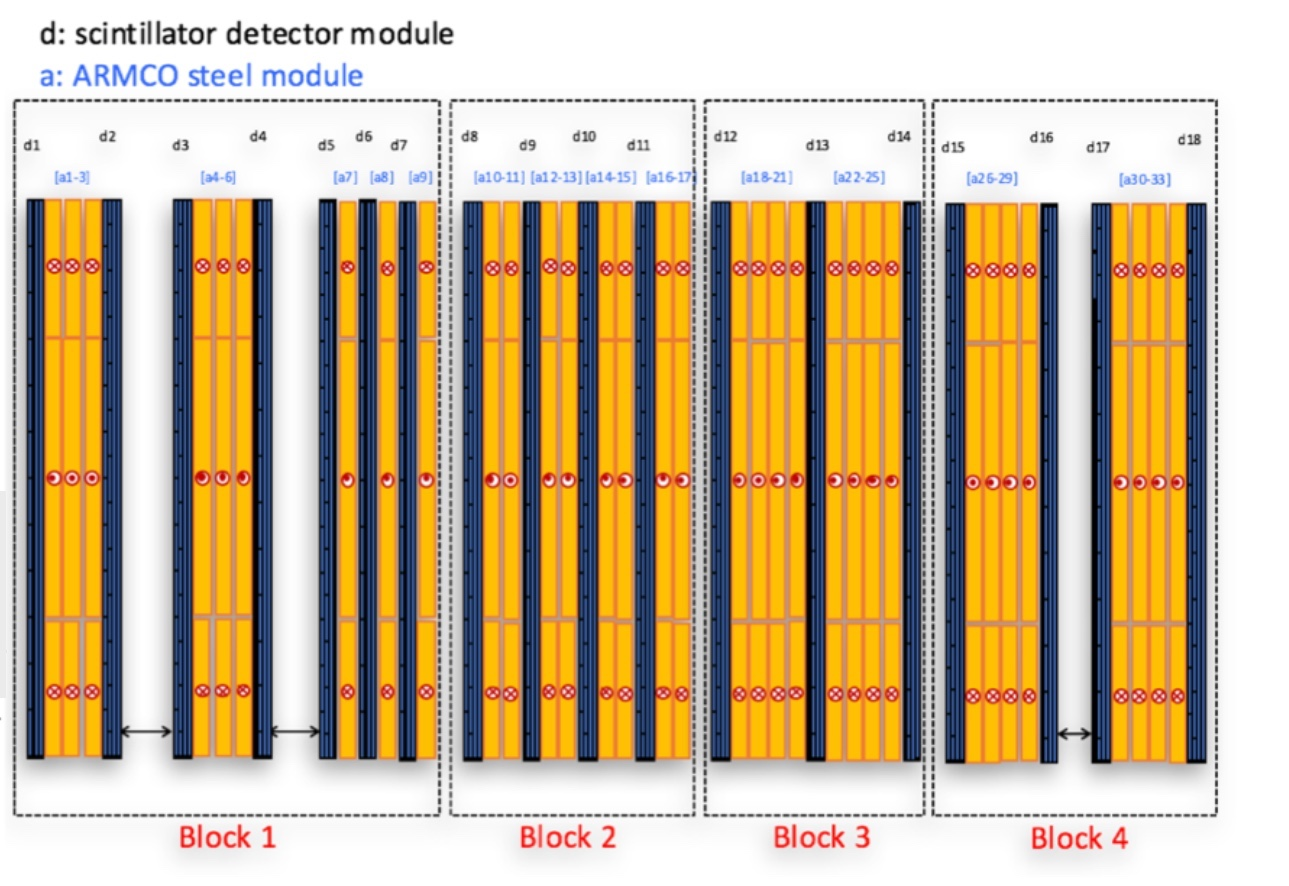
\includegraphics[width=0.48\textwidth]{figures/MIND.jpeg}
%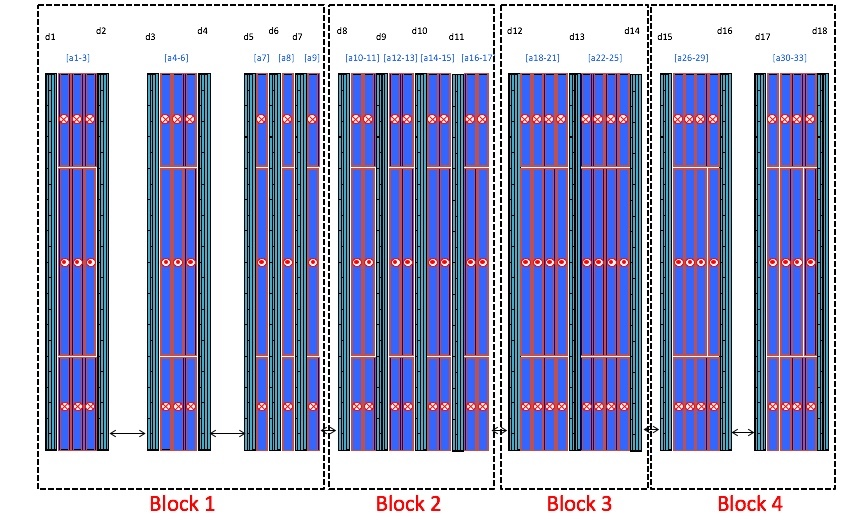
\includegraphics[width=0.48\textwidth]{figures/oldStudies/MINDetam.jpeg}
\caption{(Left) Image of the initial Baby MIND layout. (Right) The current Baby MIND layout. The main differences consists of removing the first scintillator plane, some different layout in the middle blocks and removed the final scintillator plane.}
\label{fig:oldMIND}
\end{figure}

\begin{figure}[h!]
\centering
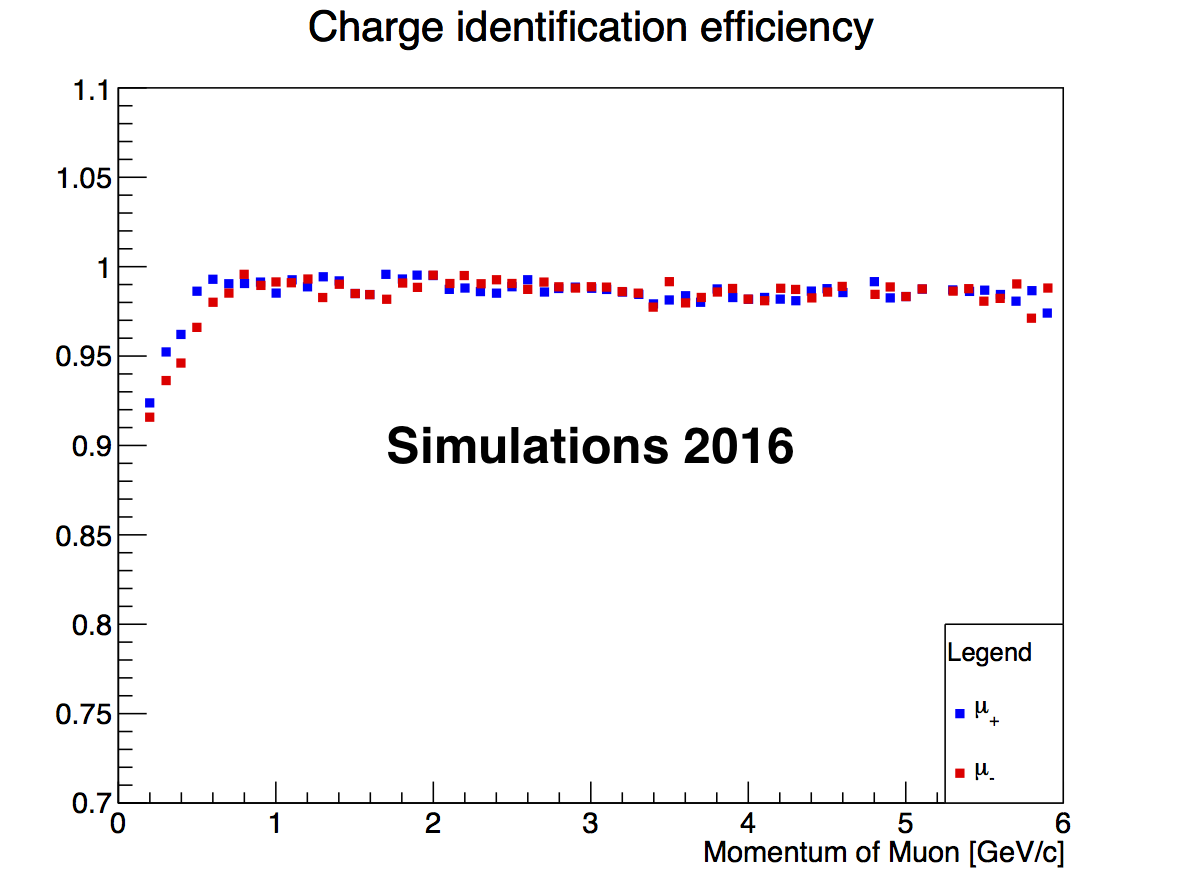
\includegraphics[width=0.48\textwidth]{figures/oldStudies/oldChargeID.png}
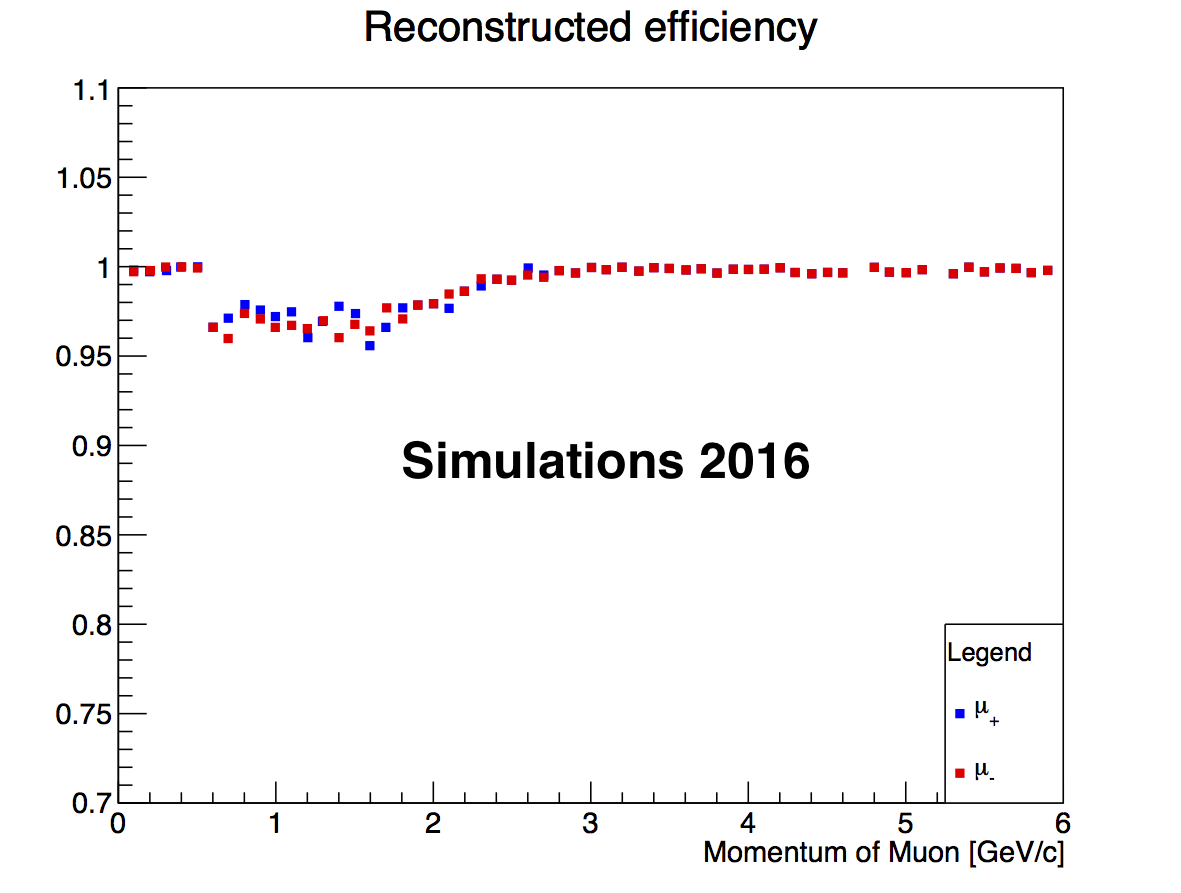
\includegraphics[width=0.48\textwidth]{figures/oldStudies/oldRecEff.png}
\caption{Metric plots of the initial Baby MIND layout with all algorithms adjusted to utilize this layout.}
\label{fig:oldMIND2}
\end{figure}

\begin{figure}[h!]
\centering
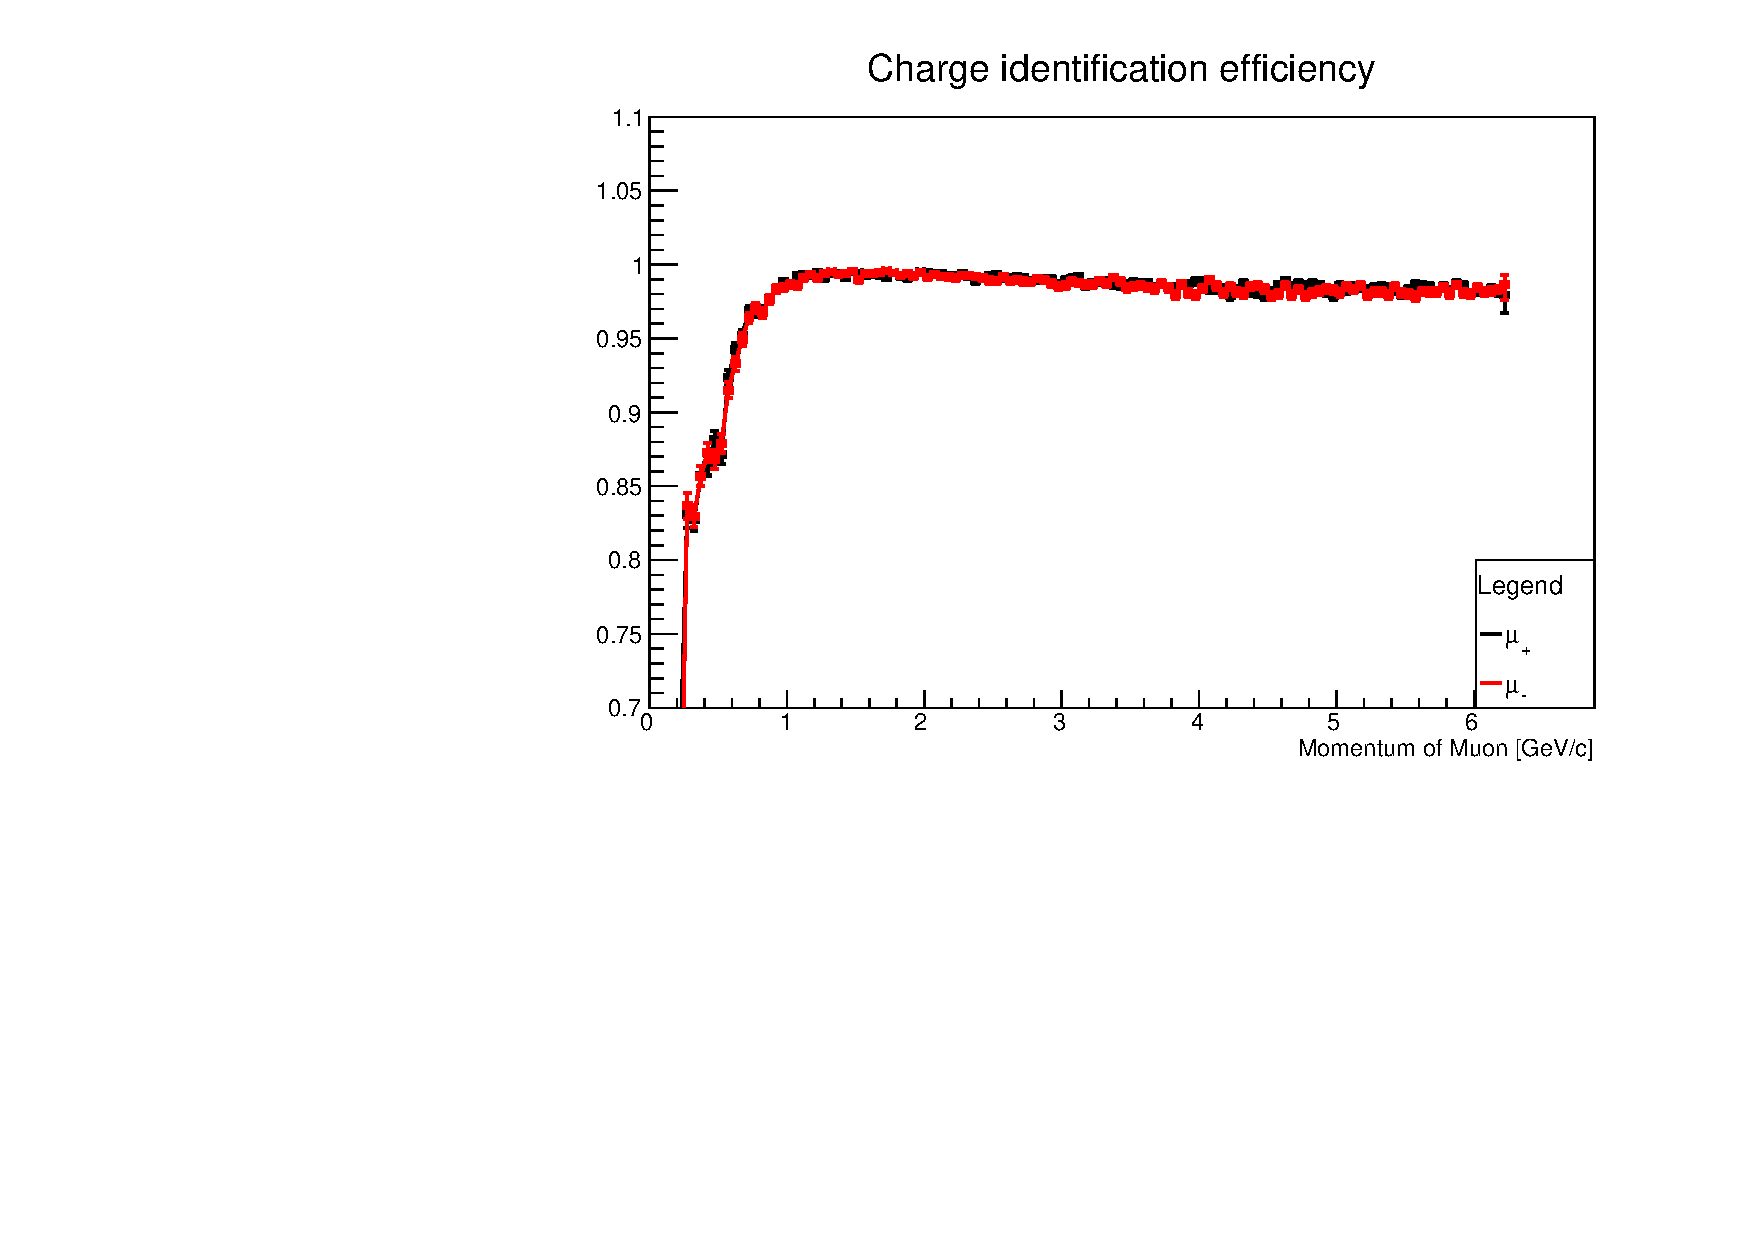
\includegraphics[width=0.48\textwidth]{figures/oldStudies/FullChargeID.pdf}
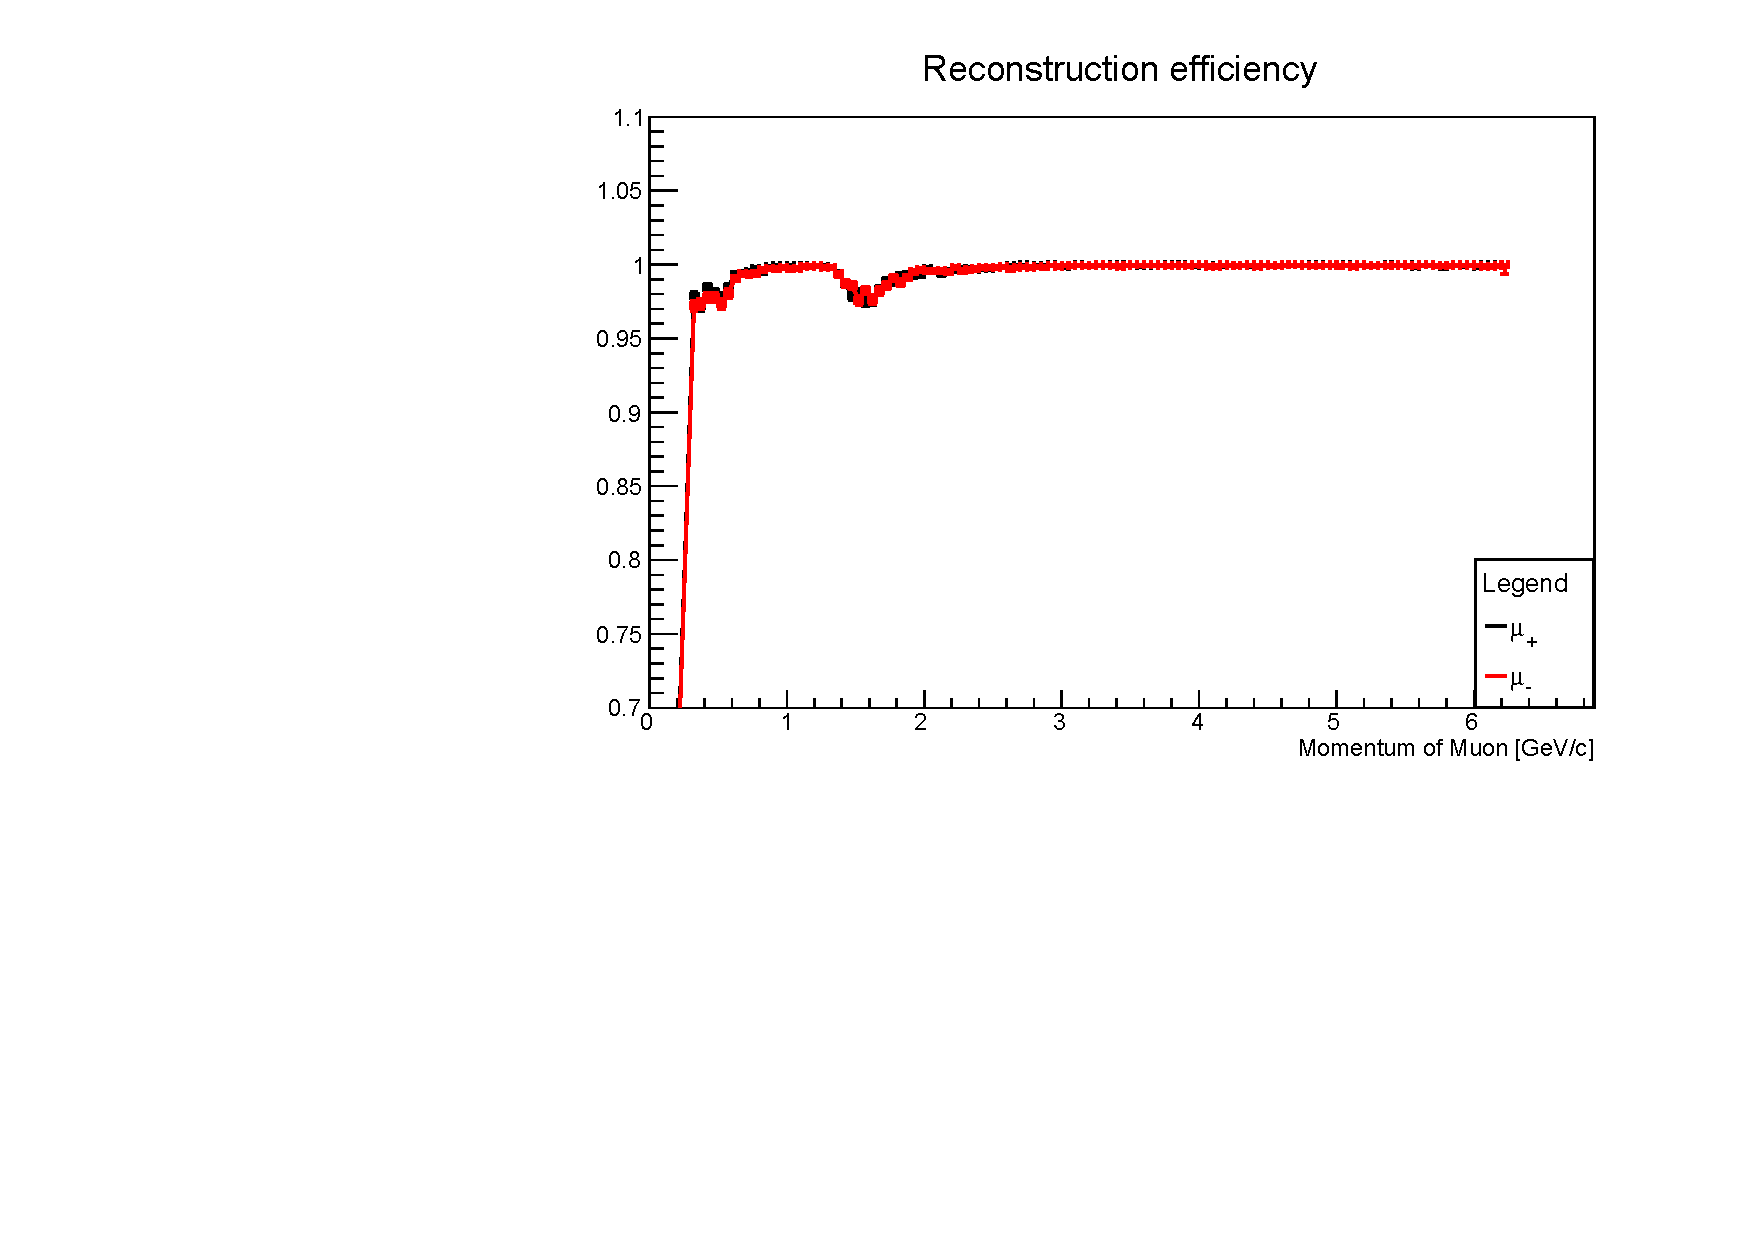
\includegraphics[width=0.48\textwidth]{figures/oldStudies/FullFitted.pdf}
\caption{Metric plots of the current Baby MIND layout.}
\label{fig:TestBeamMIND2}
\end{figure}

Give for different layouts. The initial, well worked. Then work down to the test beam layout and perhaps the latest J-parc layout? 

Charge id, fitting id, momentum pulls and so on.
Look at muons/pions. pure beams with and without TASD/WAGASCI. Especially test beam layout and J-Parc.

Add in the new layout studies?

Quite good, add that charge ID is about x for range y and so on.  Could be improved by changing layout, perhaps even tweaking algorithms etc etc but want to keep generic algorithms to handle different designs.

Momentum pulls and comparisons? Large RMS from RecPack and difficult geometry. Room for improvement.

\textbf{Perhaps cite my Uppsala proceedings?} When it is citable.

\subsection{DAQ}
Add data plots perhaps? Not sure what goes here.

Should I add details about the data format?

Explain how the unpacking works, the main data structure assumed in the electronics. The main problem with the data structure, how it is not aimed to work online. 

Read and use documentation from Yordan Ivanov Karadzhov. Also look at what Aleksander/Sascha has done and what is in the code.


\subsection{Particle identification}
Machine learning through the Toolkit for Multivariate Data Analysis with ROOT (TMVA)~\cite{TMVA}. Add some small part about what ML is and TMVA as well as some minor plots showing performances.

So far have results for $\mu^+/\mu^-$ in a background of  $\pi^+/\pi^-$. Will use for CCQE events compared to other neutrino interactions.

Currently found that the best method, however many perform similarly, is MLPBNN, Multilayer perceptron (neutral network) with BFGS training method, similar to gradient decent or quasi-Newton method, and bayesian regulator.

\subsection{Analysis software}
Start by combining, if needed, several root files. Continue by choosing interesting root branches, with or without filtering/cutting the data.
add analysis flows. What is a normal data flow? Add parts to appendix, more data etc etc etc.

Final root file, read in trees, filter out bad events, if any. Compare apples to apples. 

\section{Future development}
